\documentclass{article}
\usepackage{graphicx} % Required for inserting images
\usepackage{ctex}
\usepackage{latexsym}
\usepackage{biblatex}
\usepackage{tikz-cd}
\usepackage[toc,page]{appendix}
\addbibresource{ref.bib}
\usepackage{booktabs}
\usepackage{amsmath, amsthm, amssymb, bm, color, framed, graphicx, hyperref, mathrsfs}
\usepackage{geometry}
\usepackage[nameinlink]{cleveref}
\geometry{left=2cm,right=2cm,top=2cm,bottom=2cm}
\everymath{\displaystyle}
\title{\textbf{周周练}}
\author{Clarigatio}
\date{\today}
\linespread{1.5}
\definecolor{shadecolor}{RGB}{241, 241, 255}
\newcounter{problemname}
\newenvironment{problem}{\begin{shaded}\stepcounter{problemname}\par\noindent\textbf{Problem }}{\end{shaded}\par}
\newenvironment{solution}{\par\noindent\textbf{解答. }}{\par}
\newenvironment{lemma}{\par\noindent\textbf{引理. }}{\par}
\newenvironment{lemmasolution}{\par\noindent\textbf{引理的证明. }}{\par}
\newenvironment{note}{\par\noindent\textbf{注记. }}{\par}
\begin{document}
\maketitle
\tableofcontents
\newpage
\section*{前言}
对于较为简单的问题, 我们一般只给出答案或仅简要叙述思路, 而对于较难的问题我们一般书写详细步骤. 对周周练中的内容或其他任何数学方面的内容有疑问, 或有意向参加大学生数学竞赛的同学, 可以加我的QQ:422276215私聊, 或者线下到学支屋讨论(我一般周三下午有空, 如果要约的话请QQ上提前告知一下我).\par
一般而言, A组题比较容易, B组题属于中档题, 而C组题比较困难. 标星号$\star$的问题很困难, 甚至独立完成是不现实的. 我们鼓励读者通过查阅资料来完成这些题目.\par
\newpage
\part{题目部分}
我们在这里做一些记号上的说明. 对于常用的记号我们不在此处罗列, 而对于一些出于笔者习惯而导致与课本符号不同的情形, 读者可以查阅下面的列表.
\begin{enumerate}
    \item 我们用$\mathrm{M}_{n\times m}(\mathbb{F})$表示全体数域$\mathbb{F}$上的$n\times m$阶矩阵所构成的集合. 特别地, 用$\mathrm{M}_n(\mathbb{F})$表示全体数域$\mathbb{F}$上的$n$阶方阵. 用$\mathrm{GL}_n(\mathbb{F})$表示全体数域$\mathbb{F}$上的可逆$n$阶矩阵.
    \item 我们用$\mathrm{rank}A$表示矩阵$A$的秩.
    \item 我们用$\log$表示以$e$为底的对数(即通常意义下的$\ln$).
\end{enumerate}
\newpage
\section{第一次周练}
\subsection{数分部分}
\begin{problem}{A}\par
\begin{enumerate}
    \item 求积分$I_1=\int e^{ax}\cos bx\mathrm{d}x$和$I_2=\int e^{ax}\sin bx\mathrm{d}x$, 这里$a,b$是常数.
    \item 证明: 若$f$在$[a,b]$上可积, $F$在$[a,b]$上连续, 且除了有限个点外有$F^\prime(x)=f(x)$, 证明
    $$F(b)-F(a)=\int_a^bf(x)\mathrm{d}x.$$
\end{enumerate}
\end{problem}
\begin{problem}{B}\par
$\mathbb{R}^n$种无限多个开集的交是否一定是开集?
\end{problem}
\begin{problem}{C}\par
我们称$\mathbb{R}^n$中的一个子集$\Omega$是\textit{紧集}, 如果对任意$\Omega$的一个开覆盖$\{O_i\}_{i\in I}$都存在一个有限子覆盖$\{O_j\}_{j=1}^n\subset\{O_i\}_{i\in I}$.
\begin{enumerate}
    \item 说明开区间$(0,1)$在$\mathbb{R}$中不紧;
    \item 证明紧集的闭子集也是紧集;
    \item 证明$\mathbb{R}^n$中的紧集和有界闭集等价.
\end{enumerate}
\end{problem}
\begin{note}
我们对紧集的定义做一点说明. 所谓$\Omega$的一个开覆盖$\{O_i\}_{i\in I}$指的是每个$O_i$都是$\mathbb{R}^n$中开集, 且$\bigcup_{i\in I}O_i\supset\Omega$. 所谓$\{O_i\}_{i\in I}$的一个有限子覆盖指的是集合$\{O_i\}_{i\in I}$的有限子集.
\end{note}
\newpage
\subsection{高代部分}
\begin{problem}{A}\par
设$A_n$是$n$阶反对称矩阵, $n$为奇数, 证明$A_n$的行列式为$0$.
\end{problem}
\begin{problem}{B}\par
设$W_1$和$W_2$分别为齐次线性方程组$x_1+x_2+\cdots+x_n=0$和$x_1=x_2=\cdots=x_n$的解空间, 证明$\mathbb{R}^n=W_1\oplus W_2$.
\end{problem}
\begin{problem}{C}\par
\begin{enumerate}
    \item 设$n\ge 3$. 定义矩阵$A=(a_{ij})_{n\times n}$, 其满足
    $$
    a_{ij}=\left\{ \begin{aligned}
	a&,\left( i\ne j \right)\\
	1&,\left( i=j \right)\\
    \end{aligned} \right. 
    $$
    求$a$使得$\mathrm{dim}\mathrm{Ker}A=1$.
    \item ($\star$)对$n\ge 2$, 证明多项式$f(x)=x^n-x-1$在$\mathbb{Q}[x]$上不可约.
\end{enumerate}
\end{problem}
\begin{note}
第2题即为是Selmer定理. Selmer在1956年首次证明了这个多项式的不可约性, 其初始论文用到了算术几何的一些知识. 后来人们给出了初等的证明方法, 读者可以参考\textcolor{red}{\href{https://hydre05236.github.io/2024/03/18/Selmer-s-Theorem-on-Irreducible-Polynomials/}{笔者的这篇博客文章}}.
\end{note}
\newpage
\section{第二次周练}
\subsection{数分部分}
\begin{problem}{A}\par
\begin{enumerate}
    \item 计算$I=\int_0^{\pi/2}\sin x\log\sin x\mathrm{d}x$.
    \item 计算$\int_0^n(x-\lfloor x\rfloor)\mathrm{d}x$.
\end{enumerate}
\end{problem}
\begin{problem}{B}\par
设$V$为$\mathbb{R}^n$中的集合, 我们称$V$是一个\textit{凸集}, 如果对任意的$x_1,x_2\in V$以及$0\le t\le 1$, 成立$tx_1+(1-t)x_2\in V$. 
\begin{enumerate}
    \item 证明$\mathbb{R}^n$中的单位球$B=\{x\in\mathbb{R}^n:\|x\|\le 1\}$是凸的, 这里$\|x\|$是$x$的Euclid距离.
    \item 试证明如果$V$是凸集, 那么$V$的闭包$\bar{V}$也是凸集.
\end{enumerate}
\end{problem}
\begin{problem}{C}\par
设$f:\mathbb{R}\to\mathbb{R}$, 且有$f(x+y)=f(x)+f(y)$, 其中$x,y\in\mathbb{R}$.
\begin{enumerate}
    \item 如果$f$在至少一点处连续, 求$f$的解析式.
    \item 如果$f$在至少一点处不连续, 试证明$f$的图像$G_f=\{(x,f(x)):x\in\mathbb{R}\}$在$\mathbb{R}^2$中稠密.
\end{enumerate}
\end{problem}
\newpage
\subsection{高代部分}
\begin{problem}{A}\par
计算矩阵$
A=\left( \begin{matrix}
	2&		3\\
	1&		4\\
\end{matrix} \right) 
$的全部特征值和特征向量.
\end{problem}
\begin{problem}{B}\par
设$A=\left( \begin{matrix}
	1&		4&		2\\
	0&		-3&		4\\
	0&		4&		3\\
\end{matrix} \right) $, 求$A^k$, 这里$k$是正整数.
\end{problem}
\begin{problem}{C}\par
设$A=(a_{ij})_{m\times n},B=(b_{ij})_{r\times s}$是两个矩阵, 我们定义矩阵$A$和$B$的\textit{Kronecker积}为
$$
A\otimes B=\left( \begin{matrix}
	a_{11}B&		a_{12}B&		\cdots&		a_{1n}B\\
	a_{21}B&		a_{22}B&		\cdots&		a_{2n}B\\
	\vdots&		\vdots&		&		\vdots\\
	a_{m1}B&		a_{m2}B&		\cdots&		a_{mn}B\\
\end{matrix} \right) .
$$
下面设$A\in\mathrm{M}_n(\mathbb{R})$, $B\in\mathrm{M}_m(\mathbb{R})$.
\begin{enumerate}
    \item 证明: $A\otimes B=(A\otimes E_m)(E_n\otimes B)$.
    \item 证明: $\det(A\otimes B)=|A|^m|B|^n$.
\end{enumerate}
\end{problem}
\newpage
\section{第三次周练}
\subsection{数分部分}
\begin{problem}{A}\par
\begin{enumerate}
    \item 如果$x+y+z=e^{-(x+y+z)}$, 求$z$关于$x$, $y$的偏导数.
    \item 求极值: $f(x,y,z,t)=x+y+z+t$, 其中$xyzt=c^4$, 这里$x,y,z,t,c>0$.
\end{enumerate}
\end{problem}
\begin{problem}{B}\par
\begin{enumerate}
    \item 设$f(x,y)$在点$p_0:(x_0,y_0)$连续, 求
    $$
    \lim_{\rho \rightarrow 0} \frac{1}{\pi \rho ^2}\iint\limits_{\left( x-x_0 \right) ^2+\left( y-y_0 \right) ^2\le \rho ^2}{f\left( x,y \right) \mathrm{d}x\mathrm{d}y}.
    $$
    \item 设$f(x,y),g(x,y)$都是区域$D$上的可积函数, 证明$h(x,y)=\max\{f(x,y),g(x,y)\}$也是$D$上的可积函数.
\end{enumerate}
\end{problem}
\begin{problem}{C}\par
($\star$)设$f$, $g$都是$[0,1]$上的黎曼可积函数, 证明存在区间$[a,b]\subset[0,1]$使得
$$
\int_a^bf(x)\mathrm{d}x=\int_a^bg(x)\mathrm{d}x=\frac{1}{2}.
$$
\end{problem}
\newpage
\subsection{高代部分}\par
\begin{problem}{A}\par
\begin{enumerate}
    \item 若$n$阶方阵$A$满足$A^2+A=2E$, 问$A$是否可对角化?
    \item 设$V=\mathbb{R}^4$, 在标准内积下求$\alpha=(2,1,3,2)^\mathrm{T}$与$\beta=(1,2,-2,1)^\mathrm{T}$之间的夹角.
\end{enumerate}
\end{problem}
\begin{problem}{B}\par
求$A=\left( \begin{matrix}
	1&		0&		2\\
	0&		2&		0\\
	1&		1&		2\\
\end{matrix} \right) $的QR分解.
\end{problem}
\begin{problem}{C}\par
\textbf{本题假定读者知道Jordan标准型的相关结论.}\par
设$A$是数域$\mathbb{F}$上的一个$n$阶矩阵, 记$C(A)$为和$A$可交换的矩阵空间, 证明: 如果存在一个矩阵$X$和全部$C(A)$可交换, 那么一定存在数域$\mathbb{F}$上的一个多项式$p$, 使得$X=p(A)$.
\end{problem}
\begin{note}
本题中的结论被称为\textbf{双中心化子定理}.
\end{note}
\newpage
\section{第四次周练}
\subsection{数分部分}
\begin{problem}{A}\par
\begin{enumerate}
    \item 计算$I=\iint\limits_D{\left| x^2+y^2-4 \right|\mathrm{d}\sigma}$,其中$D=\left\{ \left( x,y \right) :x^2+y^2\le 16 \right\} $.
    \item 计算$I=\iint\limits_D{\sqrt{x^2+y^2}\mathrm{d}\sigma}$,其中$D$为$x^2+y^2=2x$围成的区域.
\end{enumerate}
\end{problem}
\begin{problem}{B}\par
证明$\int_a^b{f\left( x \right) \mathrm{d}x}\int_a^b{\frac{\mathrm{d}x}{f\left( x \right)}}\ge \left( b-a \right) ^2$,其中$f$是$[a,b]$上的正的连续函数.
\end{problem}
\begin{problem}{C}\par
设$u\in C_c^1(\mathbb{R}^3)$, 即$u\in C^1(\mathbb{R}^3)$且$u$在一个充分大的球外取值恒为$0$. 对$1\le p<3$, 证明
$$
\iiint_{\mathbb{R} ^3}{\left| u \right|^{\frac{3p}{3-p}}\mathrm{d}V}\le \left( \frac{2p}{3-p} \right) ^{\frac{3p}{2-p}}\left( \iiint_{\mathbb{R} ^3}{\left\| \nabla u \right\| ^p\mathrm{d}V} \right) ^{\frac{3}{3-p}}.
$$
\end{problem}
\begin{note}
本题的结果为\textbf{Sobolev不等式}, 其在偏微分方程中有重要作用.
\end{note}
\newpage
\subsection{高代部分}
\begin{problem}{A}\par
求正交矩阵$Q$, 使得$Q^{-1}AQ$成为对角矩阵, 其中
$$
A=\left( \begin{matrix}
	2&		-2&		0\\
	-2&		1&		2\\
	0&		-2&		0\\
\end{matrix} \right) .
$$
\end{problem}
\begin{problem}{B}\par
说明酉矩阵的行列式的模长为$1$.
\end{problem}
\begin{problem}{C}\par
设$V$是有限维Euclid空间, $V_1,V_2$是$V$的非平凡子空间, 且$V=V_1\oplus V_2$. 若$p_1,p_2$是$V_1,V_2$的正交投影, 且$\varphi=p_1+p_2$, 证明$0<\det\varphi\le 1$, 且$\det\varphi=1$当且仅当$V_1$和$V_2$正交.
\end{problem}
\newpage
\section{第五次周练}
\subsection{数分部分}
\begin{problem}{A}\par
判断下列级数收敛性:
\begin{enumerate}
    \item $$
    \sum_{n=2}^{\infty}{\frac{1}{\left( \log n \right) ^{\log n}}};
    $$
    \item $$
    \sum_{n=1}^{\infty}{\left( 1-\cos \frac{1}{n} \right)}.
    $$
\end{enumerate}
\end{problem}
\begin{problem}{B}\par
计算
$$
\sum_{n=1}^{\infty}{\left( -1 \right) ^{n+1}\frac{2n+1}{n\left( n+1 \right)}}.
$$
\end{problem}
\begin{problem}{C}\par
计算
$$
\sum_{m=1}^{\infty}{\sum_{n=1}^{\infty}{\frac{m^2n}{3^m\left( n\cdot 3^m+m\cdot 3^n \right)}}}.
$$
\end{problem}
\newpage
\subsection{高代部分}
\begin{problem}{A}\par
证明: 线性空间$V$上的双线性函数$f(\alpha,\beta)$为反称的充要条件为对任意$\alpha\in V$都有$f(\alpha,\alpha)=0$.
\end{problem}
\begin{problem}{B}\par
如果$\lambda$是正交矩阵$Q$的特征值, 证明$\lambda^{-1}$也是它的特征值.
\end{problem}
\begin{problem}{C}\par
记
$$
\mathscr{S} =\left\{ \left( \begin{matrix}
	x&		y\\
	z&		w\\
\end{matrix} \right) \in \mathrm{M}_2\left( \mathbb{R} \right) :x,y,z,w\text{构成等差数列} \right\} .
$$
求所有$C\in\mathscr{S}$, 使得对任意的$k\ge 2$, 都有$C^k\in\mathscr{S}$.
\end{problem}
\newpage
\section{第六次周练}
\subsection{数分部分}
\begin{problem}{A}\par
判断下列级数的敛散性:
\begin{enumerate}
    \item $$
\sum_{n=1}^{\infty}{\frac{\sin nx}{n^{\alpha}}},x\in \left( 0,2\pi \right) ,\alpha >0
$$
    \item $$
\sum_{n=1}^{\infty}{\frac{\left( -1 \right) ^n\log \left( n+1 \right)}{n+1}}.
$$
\end{enumerate}
\end{problem}
\begin{problem}{B}\par
设$\sum_{n=1}^\infty u_n$满足$\frac{u_{n+1}}{u_n}<1$, 能否说明$\sum_{n=1}^\infty u_n$收敛?
\end{problem}
\begin{problem}{C}\par
讨论$\sum_{n=1}^\infty\frac{(-1)^{\lfloor n^\alpha\rfloor}}{n^\beta}$的敛散性.
\end{problem}
\newpage
\subsection{高代部分}
\begin{problem}{A}\par
设$A$是$n$阶实对称矩阵且$|A|<0$, 证明:存在实$n$维列向量$X\ne 0$, 使得$X^{\mathrm{T}AX}<0$.
\end{problem}
\begin{problem}{B}\par
如果$A$是正定矩阵, 证明$A^{-1}$也是正定矩阵.
\end{problem}
\begin{problem}{C}\par
证明: 一族两两可交换奇数阶实矩阵必有公共特征向量.
\end{problem}
\newpage
\part{答案部分}
\newpage
\section{第一次周练}
\subsection{数分部分}
\begin{problem}{A}\par
\begin{enumerate}
    \item 求积分$I_1=\int e^{ax}\cos bx\mathrm{d}x$和$I_2=\int e^{ax}\sin bx\mathrm{d}x$, 这里$a,b$是常数.
    \item 证明: 若$f$在$[a,b]$上可积, $F$在$[a,b]$上连续, 且除了有限个点外有$F^\prime(x)=f(x)$, 证明
    $$F(b)-F(a)=\int_a^bf(x)\mathrm{d}x.$$
\end{enumerate}
\end{problem}
\begin{solution}
\begin{enumerate}
    \item 注意到
    $$
    I_1=\frac{1}{a}\int{\cos bx\mathrm{d}\left( e^{ax} \right)}=\frac{1}{a}\left( e^{ax}\cos bx+bI_2 \right) 
    $$
    以及
    $$
    I_2=\frac{1}{a}\int{\sin bx\mathrm{d}\left( e^{ax} \right)}=\frac{1}{a}\left( e^{ax}\sin bx-bI_1 \right) ,
    $$
    我们有关于$I_1$和$I_2$的线性方程组, 解得
    $$
    I_1=\frac{b\sin bx+a\cos bx}{a^2+b^2}e^{ax}+C;\hspace{0.5cm}I_2=\frac{a\sin bx-b\cos bx}{a^2+b^2}e^{ax}+C.
    $$
    \item 对$[a,b]$做分割$T$, 使得不满足$F^\prime(x)=f(x)$的有限个点恒为$T$中的一个部分分点. 此时在每个小区间$[x_{i-1},x_i]$上$F$满足微分中值定理条件, 从而存在$\xi_i\in (x_{i-1},x_i)$使得
    $$
    F\left( x_i \right) -F\left( x_{i-1} \right) =F^{\prime}\left( \xi _i \right) \left( x_i-x_{i-1} \right) =f\left( \xi _i \right) \left( x_i-x_{i-1} \right) .
    $$
    因此
    $$
    \int_a^b{f\left( x \right) \mathrm{d}x}=\lim_{n\rightarrow \infty} \sum_{i=1}^n{f\left( \xi _i \right) \left( x_i-x_{i-1} \right)}=\lim_{n\rightarrow \infty} \sum_{i=1}^n{F^{\prime}\left( \xi _i \right) \left( x_i-x_{i-1} \right)}=F\left( b \right) -F\left( a \right) .
    $$
\end{enumerate}
\end{solution}
\begin{problem}{B}\par
$\mathbb{R}^n$种无限多个开集的交是否一定是开集?
\end{problem}
\begin{solution}
不一定. 考虑$\bigcap_{n=1}^\infty\left(1+\frac{1}{n},2\right)$.
\end{solution}
\begin{problem}{C}\par
我们称$\mathbb{R}^n$中的一个子集$\Omega$是\textit{紧集}, 如果对任意$\Omega$的一个开覆盖$\{O_i\}_{i\in I}$都存在一个有限子覆盖$\{O_j\}_{j=1}^n\subset\{O_i\}_{i\in I}$.
\begin{enumerate}
    \item 说明开区间$(0,1)$在$\mathbb{R}$中不紧;
    \item 证明紧集的闭子集也是紧集;
    \item 证明$\mathbb{R}^n$中的紧集和有界闭集等价.
\end{enumerate}
\end{problem}
\begin{solution}
\begin{enumerate}
    \item 记$O_n=\left(0,1-\frac{1}{n}\right)$, 考虑开覆盖$\{O_n\}_{n=1}^\infty$.
    \item 设$K$是一个紧集, $V$是$K$的一个闭子集. 设$\{O_\lambda\}_{\lambda\in I}$为$V$的任意一个开覆盖, 则$\{O_\lambda\}$与$V^c$一起形成$K$的一个开覆盖, 而$K$是紧集, 因此存在有限开覆盖, 记为$\{O_1,\cdots,O_{k-1},V^c\}$. 不妨设$V^c=O_k$, 由于$V\subset K$, 我们有
    $$
    \left( \bigcup_{i=1}^{k-1}{O_k} \right) \cup V^c\supset K\supset V.
    $$
    但$V^c\cap V=\emptyset$, 故$\bigcap_{i=1}^{k-1}O_i\supset V$, 这就完成了证明.
    \item 以下的讨论都在$\mathbb{R}^n$中进行(赋予$\mathbb{R}^n$上的通常拓扑). 设$K$是紧集, 我们证明$K$是有界闭集. 我们首先证明$K$的任意一个无限子集必有聚点落在$K$中. 设若不然, 记$F$为$K$的一个无限子集, 但对任意$x\in K$都有$x$不是$F$的聚点. 由聚点的定义, 存在$\delta_x>0$, 使得在$x$的一个$\delta_x$-邻域$U(x,\delta_x)$中没有异于$x$的$F$中的点. 注意到$\{U(x,\delta_x)\}_{x\in K}$构成了$K$的一个开覆盖, 因此由$K$紧知存在$\{U(x_i,\delta_i)\}_{i=1}^n$是$K$的一个有限子覆盖. 然而这导致$F$是一个有限集, 矛盾! 因此$K^\circ\subset K$, 从而为闭集. 下面只要证明$K$是有限集. 设若不然, $K$中有子列$\{x_k\}$满足$x_k\to\infty$, 从而$\{x_k\}$没有聚点, 这是一个矛盾!\par
    反过来, 注意到任意一个有界闭集都可以被$\mathbb{R}^n$中的一个充分大的闭矩形覆盖, 显然闭矩形是紧的, 而紧集的闭子集也是紧集, 这就完成了证明.
\end{enumerate}
\end{solution}
\begin{note}
我们对第三问做一些补充说明. 关于$\mathbb{R}^n$中的闭矩形是紧的的证明可以使用闭球套定理(事实上为一维情形的Borel覆盖定理的推广). 另一个思路是由Borel覆盖定理知$\mathbb{R}$中的闭区间是紧的, 如果我们能够证明紧集的乘积也是紧的, 那么只要将$\mathbb{R}^n$中的闭矩形拆成$n$个$\mathbb{R}$中的闭区间的乘积即可. 事实上这是成立的, 吉洪诺夫定理保证了任意多个紧集的乘积仍然是紧集. 但这里涉及到很多细节(例如$\mathbb{R}^n$上的拓扑定义为$n$个$\mathbb{R}$的乘积的拓扑的合理性等), 我们不再展开, 感兴趣的读者参考尤承业乘积拓扑部分, 以及Munkres中吉洪诺夫定理的证明部分.
\end{note}
\newpage
\subsection{高代部分}
\begin{problem}{A}\par
设$A_n$是$n$阶反对称矩阵, $n$为奇数, 证明$A_n$的行列式为$0$.
\end{problem}
\begin{solution}
由题意知$A^{\mathrm{T}}=-A$, 两边取行列式有$|A|=(-1)^n|A|$, 由于$n$是奇数, 因此$|A|=-|A|$, 从而$|A|=0$, 证毕.
\end{solution}
\begin{problem}{B}\par
设$W_1$和$W_2$分别为齐次线性方程组$x_1+x_2+\cdots+x_n=0$和$x_1=x_2=\cdots=x_n$的解空间, 证明$\mathbb{R}^n=W_1\oplus W_2$.
\end{problem}
\begin{solution}
显然$x_1+x_2+\cdots+x_n=0$的解空间是$n-1$维的, 且
$$
e_1=\left( 1,-1,0,\cdots ,0 \right) ^{\mathrm{T}};\hspace{0.2cm}e_2=\left( 1,0,-1,\cdots ,0 \right) ^{\mathrm{T}};\hspace{0.2cm}\cdots \hspace{0.2cm}e_{n-1}=\left( 1,0,0,\cdots ,-1 \right) ^{\mathrm{T}}
$$
为$W_1$的一个基. 又$x_1=x_2=\cdots=x_n$的解空间为$1$维的, 且$e_n=(1,1,\cdots,1)^{\mathrm{T}}$为$W_2$的一个基, 因此只要证明$e_1,\cdots,e_n$线性无关. 而
$$
\left| \begin{matrix}
	-1&		-1&		\cdots&		-1&		1\\
	1&		0&		\cdots&		0&		1\\
	0&		1&		\cdots&		0&		1\\
	\vdots&		\vdots&		&		\vdots&		\vdots\\
	0&		0&		\cdots&		1&		1\\
\end{matrix} \right|=\left( -1 \right) ^{n+1}\ne 0,
$$
这就完成了证明.
\end{solution}
\begin{problem}{C}\par
\begin{enumerate}
    \item 设$n\ge 3$. 定义矩阵$A=(a_{ij})_{n\times n}$, 其满足
    $$
    a_{ij}=\left\{ \begin{aligned}
	a&,\left( i\ne j \right)\\
	1&,\left( i=j \right)\\
    \end{aligned} \right. 
    $$
    求$a$使得$\mathrm{dim}\mathrm{Ker}A=1$.
    \item ($\star$)对$n\ge 2$, 证明多项式$f(x)=x^n-x-1$在$\mathbb{Q}[x]$上不可约.
\end{enumerate}
\end{problem}
\begin{solution}
\begin{enumerate}
    \item 若$\mathrm{dim}\mathrm{Ker}A=1$, 那么方程$Ax=0$有非零解, 从而$|A|=0$. 下面我们计算$|A|$. 事实上
    $$
    \begin{aligned}
    \left| A \right|&=\left| \begin{matrix}
	a&		1&		\cdots&		1\\
	1&		a&		\cdots&		1\\
	\vdots&		\vdots&		\ddots&		\vdots\\
	1&		1&		\cdots&		a\\
    \end{matrix} \right|=\left| \begin{matrix}
	a+n-1&		1&		\cdots&		1\\
	a+n-1&		a&		\cdots&		1\\
	\vdots&		\vdots&		\ddots&		\vdots\\
	a+n-1&		1&		\cdots&		a\\
    \end{matrix} \right|=\left( a+n-1 \right) \left| \begin{matrix}
	1&		1&		\cdots&		1\\
	1&		a&		\cdots&		1\\
	\vdots&		\vdots&		\ddots&		\vdots\\
	1&		1&		\cdots&		a\\
    \end{matrix} \right|
    \\
    &=\left( a+n-1 \right) \left| \begin{matrix}
	1&		1&		\cdots&		1\\
	0&		a-1&		\cdots&		0\\
	\vdots&		\vdots&		\ddots&		\vdots\\
	0&		0&		\cdots&		a-1\\
    \end{matrix} \right|=\left( a+n-1 \right) \left( a-1 \right) ^{n-1},
    \end{aligned}
    $$
    从而$a=1$或$a=1-n$.\par
    若$a=1$, 那么$x=(x_1,\cdots,x_n)^{\mathrm{T}}\in\mathrm{Ker}A$当且仅当$x_1+x_2+\cdots+x_n=0$, 因此$\mathrm{dim}\mathrm{Ker}A=n-1\ge 2$, 这是一个矛盾!\par
    若$a=1-n$, 那么$x_0=(1,\cdots,1)^{\mathrm{T}}\ne 0$满足$Ax_0=0$, 且$\mathrm{rank}A=n-1$. 于是$\mathrm{dim}\mathrm{Ker}A=1$. 综上所述我们有$a=1-n$.
    \item 见{\href{https://hydre05236.github.io/2024/03/18/Selmer-s-Theorem-on-Irreducible-Polynomials/}{此文}}.
\end{enumerate}
\end{solution}
\newpage
\section{第二次周练}
\subsection{数分部分}
\begin{problem}{A}\par
\begin{enumerate}
    \item 计算$I=\int_0^{\pi/2}\sin x\log\sin x\mathrm{d}x$.
    \item 计算$\int_0^n(x-\lfloor x\rfloor)\mathrm{d}x$.
\end{enumerate}
\end{problem}
\begin{solution}
\begin{enumerate}
    \item 我们有
    $$
    \begin{aligned}
\int_0^{\pi /2}{\sin x\log \left( \sin x \right) \mathrm{d}x}&=\int_0^{\pi /2}{\log \left( \sin x \right) \mathrm{d}\left( 1-\cos x \right)}
\\
&=\left( 1-\cos x \right) \mid _{0^+}^{\pi /2}-\int_0^{\pi /2}{\left( 1-\cos x \right) \mathrm{d}\left( \log \left( \sin x \right) \right)}
\\
&=-\int_0^{\pi /2}{\left( 1-\cos x \right) \cdot \frac{\cos x}{\sin x}\mathrm{d}x}
\\
&=-\int_0^{\pi /2}{\frac{\sin x\cos x}{1+\cos x}\mathrm{d}x}
\\
&=\int_0^{\pi /2}{\left( -\sin x+\frac{\sin x}{1+\cos x} \right) \mathrm{d}x}
\\
&=\left[ \cos x-\log \left( 1+\sin x \right) \right] \mid _{0}^{\pi /2}=\log 2-1.
    \end{aligned}
    $$
    \item 我们有
    $$
\int_0^n{\left( x-\lfloor x \rfloor \right) \mathrm{d}x}=\sum_{k=1}^n{\int_{k-1}^k{\left( x-\lfloor x \rfloor \right) \mathrm{d}x}}=n\int_0^1{\left( x-\lfloor x \rfloor \right) \mathrm{d}x}=\frac{n}{2}.
    $$
\end{enumerate}
\end{solution}
\begin{problem}{B}\par
设$V$为$\mathbb{R}^n$中的集合, 我们称$V$是一个\textit{凸集}, 如果对任意的$x_1,x_2\in V$以及$0\le t\le 1$, 成立$tx_1+(1-t)x_2\in V$. 
\begin{enumerate}
    \item 证明$\mathbb{R}^n$中的单位球$B=\{x\in\mathbb{R}^n:\|x\|\le 1\}$是凸的, 这里$\|x\|$是$x$的Euclid距离.
    \item 试证明如果$V$是凸集, 那么$V$的闭包$\bar{V}$也是凸集.
\end{enumerate}
\end{problem}
\begin{solution}
对第一问, 只要按定义验证即可. 我们重点证明第二问. 任取$x,y\in\bar{V}$, 我们可以分别取一列$\{x_n\}_{n=1}^\infty, \{y_n\}_{n=1}^\infty\subset V$使得$x_n\to x$, $y_n\to y$. 因此对任意的$\lambda\in[0,1]$我们有
$$
\lim_{n\rightarrow \infty} \left[ \lambda x_n+\left( 1-\lambda \right) y_n \right] =\lambda x+\left( 1-\lambda \right) y\in \bar{V},
$$
这就完成了证明.
\end{solution}
\begin{problem}{C}\par
设$f:\mathbb{R}\to\mathbb{R}$, 且有$f(x+y)=f(x)+f(y)$, 其中$x,y\in\mathbb{R}$.
\begin{enumerate}
    \item 如果$f$在至少一点处连续, 求$f$的解析式.
    \item 如果$f$在至少一点处不连续, 试证明$f$的图像$G_f=\{(x,f(x)):x\in\mathbb{R}\}$在$\mathbb{R}^2$中稠密.
\end{enumerate}
\end{problem}
\begin{solution}
\begin{enumerate}
    \item 我们可以不妨设$f$处处连续, 这是因为若$f$在$x_0$处连续, 那么
    $$
    \lim_{y\rightarrow 0} f\left( x_0+y \right) =f\left( x_0 \right) +\lim_{y\rightarrow 0} f\left( y \right) =f\left( x_0 \right) ,
    $$
    因此$\lim_{y\to 0}f(y)=0$, 从而$f$在$x=0$处连续. 类似可以证明$f$处处连续. 注意到
    $$
    f\left( nx \right) =f\left( \left( n-1 \right) x \right) +f\left( x \right) =\cdots =nf\left( x \right) ,
    $$
    用$\frac{x}{n}$代替$x$, 我们有$f\left(\frac{m}{n}x\right)=\frac{m}{n}f(x)$, 因此对任意的$r\in\mathbb{Q}$, 我们有$f(rx)=rf(x)$. 进一步利用有理数在实数中的稠密性以及$f$的连续性就有$f(x)=cx$, 这里$c$是常数.
    \item 我们用$\mathrm{cl}(A)$来表示$A$的闭包. 那么由于$f$不连续, 存在$x_0$使得$(x_0,f(x_0))$与$(1,f(1))$线性无关. 现在
    $$
    \begin{aligned}
\mathbb{R} ^2&=\left\{ a\left( 1,f\left( 1 \right) \right) +b\left( x_0,f\left( x_0 \right) \right) :a,b\in \mathbb{R} \right\} 
\\
&=\mathrm{cl}\left( \left\{ a\left( 1,f\left( 1 \right) \right) +b\left( x_0,f\left( x_0 \right) \right) :a,b\in \mathbb{Q} \right\} \right) 
\\
&=\mathrm{cl}\left( \left\{ \left( a+bx_0,f\left( a+bx_0 \right) \right) :a,b\in \mathbb{Q} \right\} \right) 
\\
&=\mathrm{cl}\left( \left\{ \left( x,f\left( x \right) \right) :x\in \mathbb{R} \right\} \right) ,
    \end{aligned}
    $$
    这就完成了证明.
\end{enumerate}
\end{solution}
\newpage
\subsection{高代部分}
\begin{problem}{A}\par
计算矩阵$
A=\left( \begin{matrix}
	2&		3\\
	1&		4\\
\end{matrix} \right) 
$的全部特征值和特征向量.
\end{problem}
\begin{solution}
矩阵$A$的两个特征值为$\lambda=5$, $\lambda=1$, 特征向量为$\zeta_1=(1,1)^\mathrm{T}$, $\zeta_2=(-3,1)^\mathrm{T}$.
\end{solution}
\begin{problem}{B}\par
设$A=\left( \begin{matrix}
	1&		4&		2\\
	0&		-3&		4\\
	0&		4&		3\\
\end{matrix} \right) $, 求$A^k$, 这里$k$是正整数.
\end{problem}
\begin{solution}
这是高代答疑群里的题目. 以下是笔者当时码的解答.
\begin{figure}[htbp]
    \center
    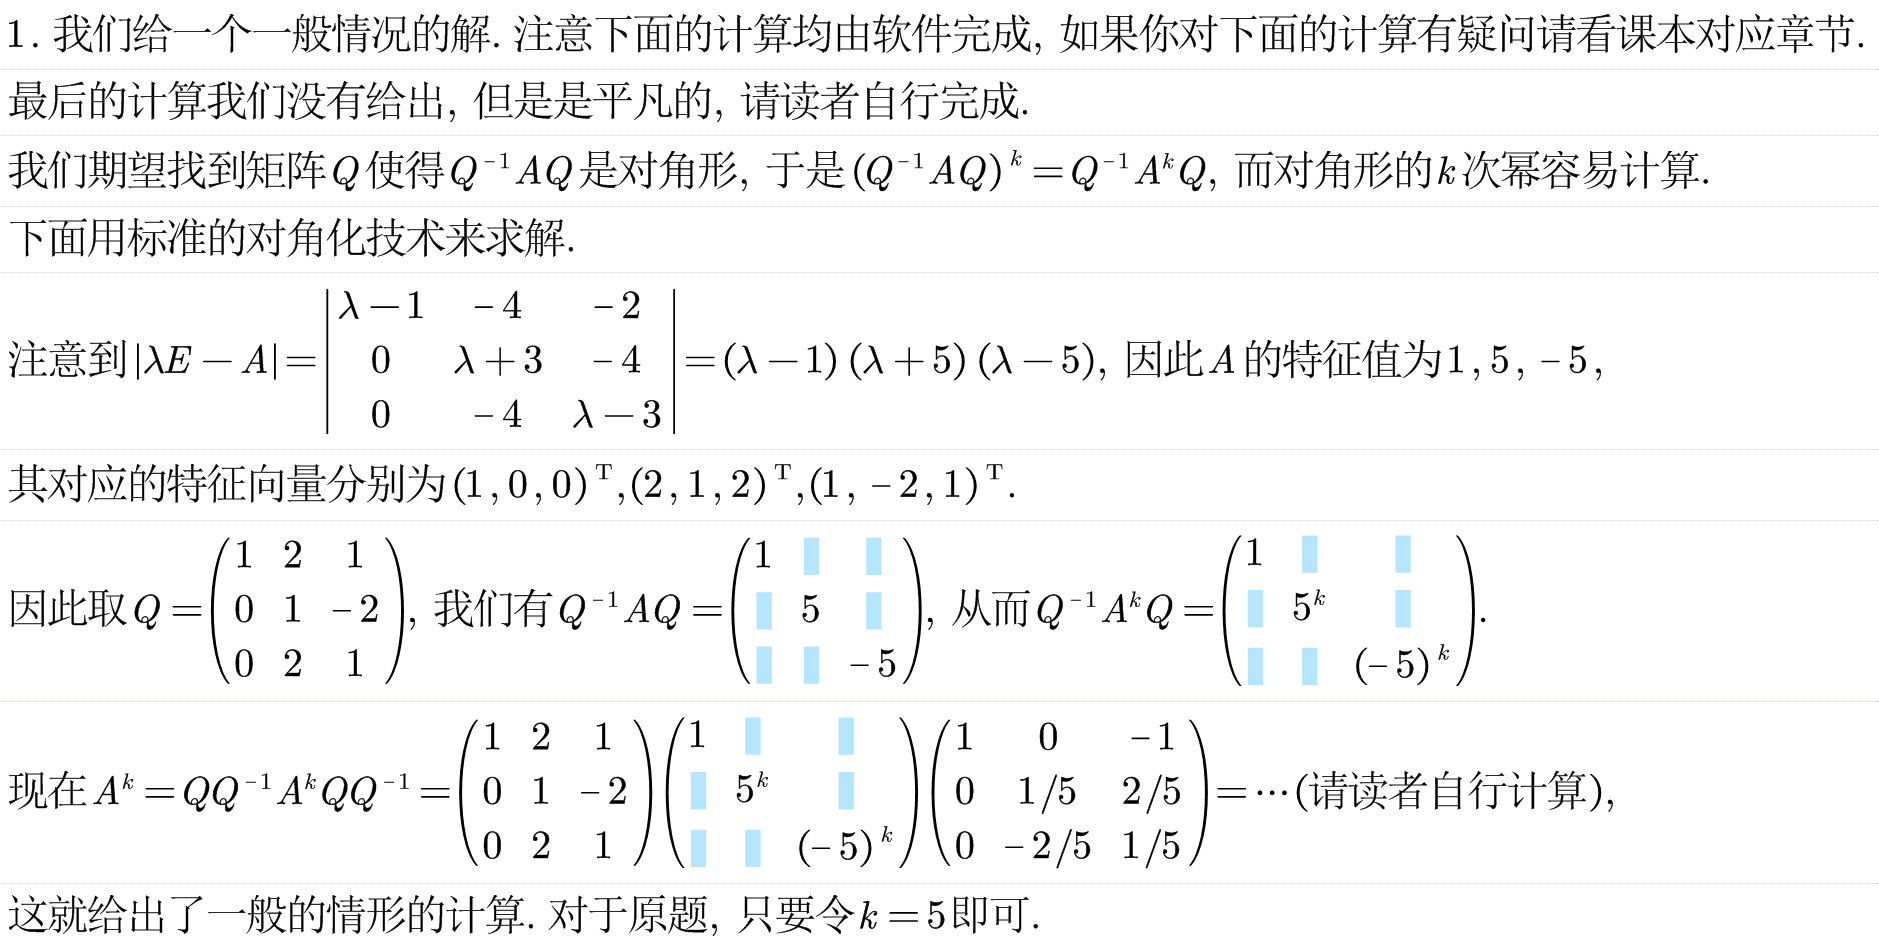
\includegraphics[scale=0.26]{1.png}
\end{figure}
\end{solution}
\begin{problem}{C}\par
设$A=(a_{ij})_{m\times n},B=(b_{ij})_{r\times s}$是两个矩阵, 我们定义矩阵$A$和$B$的\textit{Kronecker积}为
$$
A\otimes B=\left( \begin{matrix}
	a_{11}B&		a_{12}B&		\cdots&		a_{1n}B\\
	a_{21}B&		a_{22}B&		\cdots&		a_{2n}B\\
	\vdots&		\vdots&		&		\vdots\\
	a_{m1}B&		a_{m2}B&		\cdots&		a_{mn}B\\
\end{matrix} \right) .
$$
下面设$A\in\mathrm{M}_n(\mathbb{R})$, $B\in\mathrm{M}_m(\mathbb{R})$.
\begin{enumerate}
    \item 证明: $A\otimes B=(A\otimes E_m)(E_n\otimes B)$.
    \item 证明: $\det(A\otimes B)=|A|^m|B|^n$.
\end{enumerate}
\end{problem}
\begin{solution}
第一问是平凡的计算验证, 我们仅证明第二问. 由第一问的结果我们有
$$
\det \left( A\otimes B \right) =\det \left( A\otimes E_m \right) \det \left( E_n\otimes B \right) .
$$
而注意到
\begin{figure}[htbp]
    \center
    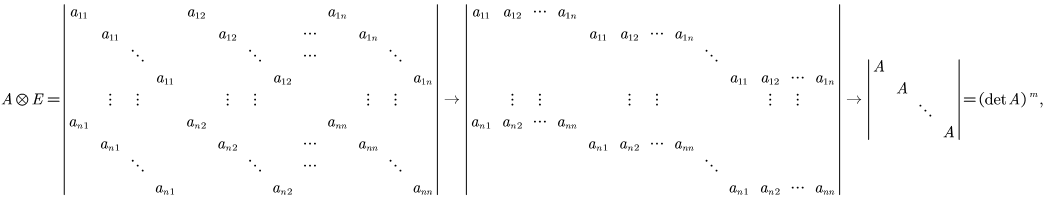
\includegraphics[scale=0.46]{2.png}
\end{figure}

同理对$E_n\otimes B$有类似结果, 我们完成了证明.
\end{solution}
\newpage
\section{第三次周练}
\subsection{数分部分}
\begin{problem}{A}\par
\begin{enumerate}
    \item 如果$x+y+z=e^{-(x+y+z)}$, 求$z$关于$x$, $y$的偏导数.
    \item 求极值: $f(x,y,z,t)=x+y+z+t$, 其中$xyzt=c^4$, 这里$x,y,z,t,c>0$.
\end{enumerate}
\end{problem}
\begin{solution}
\begin{enumerate}
    \item 令$F(x,y,z)=x+y+z-e^{-(x+y+z)}$, 则$F_x=1+e^{-\left( x+y+z \right)}=F_y=F_z$.因此$\frac{\partial z}{\partial x}=\frac{\partial z}{\partial y}=-1$.
    \item 应用Lagrange常数法可以得到极值为$f(c,c,c,c)=4c$.
\end{enumerate}
\end{solution}
\begin{problem}{B}\par
\begin{enumerate}
    \item 设$f(x,y)$在点$p_0:(x_0,y_0)$连续, 求
    $$
    \lim_{\rho \rightarrow 0} \frac{1}{\pi \rho ^2}\iint\limits_{\left( x-x_0 \right) ^2+\left( y-y_0 \right) ^2\le \rho ^2}{f\left( x,y \right) \mathrm{d}x\mathrm{d}y}.
    $$
    \item 设$f(x,y),g(x,y)$都是区域$D$上的可积函数, 证明$h(x,y)=\max\{f(x,y),g(x,y)\}$也是$D$上的可积函数.
\end{enumerate}
\end{problem}
\begin{solution}
\begin{enumerate}
    \item 由积分中值定理知存在点$(\zeta,\eta)$使得
    $$
    \iint\limits_{\left( x-x_0 \right) ^2+\left( y-y_0 \right) ^2\le \rho ^2}{f\left( x,y \right) \mathrm{d}x\mathrm{d}y}=f\left( \zeta ,\eta \right) \iint\limits_{\left( x-x_0 \right) ^2+\left( y-y_0 \right) ^2\le \rho ^2}{\mathrm{d}x\mathrm{d}y}=\pi \rho ^2f\left( \zeta ,\eta \right) .
    $$
    因此
    $$
    \lim_{\rho \rightarrow 0} \frac{1}{\pi \rho ^2}\iint\limits_{\left( x-x_0 \right) ^2+\left( y-y_0 \right) ^2\le \rho ^2}{f\left( x,y \right) \mathrm{d}x\mathrm{d}y}=\lim_{\rho \rightarrow 0} f\left( \zeta ,\eta \right) =f\left( p_0 \right) .
    $$
    \item 只要注意到$\max \left\{ f,g \right\} =\frac{f+g+\left| f-g \right|}{2}$.
\end{enumerate}
\end{solution}
\begin{problem}{C}\par
($\star$)设$f$, $g$都是$[0,1]$上的黎曼可积函数, 证明存在区间$[a,b]\subset[0,1]$使得
$$
\int_a^bf(x)\mathrm{d}x=\int_a^bg(x)\mathrm{d}x=\frac{1}{2}.
$$
\end{problem}
\begin{solution}
我们首先介绍一个引理: 对连续映射$f:\mathbb{S}^n\to\mathbb{R}^n$, 存在$X\in\mathbb{S}^n$, 使得$f(X)=f(-X)$, 这里$\mathbb{S}^n$是$\mathbb{R}^{n+1}$中的单位球面. 该定理的证明读者可以参考Hatcher:\textit{Algebraic Topology}第32页定理1.10, 并且在后面我们会给出该引理的一个初等证法. 现在我们来证明原题.\par
考虑$\mathbb{S}^2\to\mathbb{R}^2$的连续映射
\begin{small}
$$
\left( x,y,z \right) \mapsto \left( \mathrm{sgn} x\int_0^{x^2}{f\mathrm{d}t}+\mathrm{sgn} y\int_{x^2}^{x^2+y^2}{f\mathrm{d}t}+\mathrm{sgn} z\int_{x^2+y^2}^1{f\mathrm{d}t},\mathrm{sgn} x\int_0^{x^2}{g\mathrm{d}t}+\mathrm{sgn} y\int_{x^2}^{x^2+y^2}{g\mathrm{d}t}+\mathrm{sgn} z\int_{x^2+y^2}^1{g\mathrm{d}t} \right) .
$$
\end{small}
由前面的引理, 我们知道存在$(x_0,y_0,z_0)\in\mathbb{S}^2$使得
\begin{small}
$$
\mathrm{sgn} x_0\int_0^{x_{0}^{2}}{f\mathrm{d}t}+\mathrm{sgn} y_0\int_{x_{0}^{2}}^{x_{0}^{2}+y_{0}^{2}}{f\mathrm{d}t}+\mathrm{sgn} z_0\int_{x_{0}^{2}+y_{0}^{2}}^1{f\mathrm{d}t}=-\mathrm{sgn} x_0\int_0^{x_{0}^{2}}{f\mathrm{d}t}-\mathrm{sgn} y_0\int_{x_{0}^{2}}^{x_{0}^{2}+y_{0}^{2}}{f\mathrm{d}t}-\mathrm{sgn} z_0\int_{x_{0}^{2}+y_{0}^{2}}^1{f\mathrm{d}t}
$$
\end{small}
以及
\begin{small}
$$
\mathrm{sgn} x_0\int_0^{x_{0}^{2}}{g\mathrm{d}t}+\mathrm{sgn} y_0\int_{x_{0}^{2}}^{x_{0}^{2}+y_{0}^{2}}{g\mathrm{d}t}+\mathrm{sgn} z_0\int_{x_{0}^{2}+y_{0}^{2}}^1{g\mathrm{d}t}=-\mathrm{sgn} x_0\int_0^{x_{0}^{2}}{g\mathrm{d}t}-\mathrm{sgn} y_0\int_{x_{0}^{2}}^{x_{0}^{2}+y_{0}^{2}}{g\mathrm{d}t}-\mathrm{sgn} z_0\int_{x_{0}^{2}+y_{0}^{2}}^1{g\mathrm{d}t},
$$
\end{small}
于是就有
$$
\mathrm{sgn} x_0\int_0^{x_{0}^{2}}{f\mathrm{d}t}+\mathrm{sgn} y_0\int_{x_{0}^{2}}^{x_{0}^{2}+y_{0}^{2}}{f\mathrm{d}t}+\mathrm{sgn} z_0\int_{x_{0}^{2}+y_{0}^{2}}^1{f\mathrm{d}t}=0
$$
以及
$$
\mathrm{sgn} x_0\int_0^{x_{0}^{2}}{g\mathrm{d}t}+\mathrm{sgn} y_0\int_{x_{0}^{2}}^{x_{0}^{2}+y_{0}^{2}}{g\mathrm{d}t}+\mathrm{sgn} z_0\int_{x_{0}^{2}+y_{0}^{2}}^1{g\mathrm{d}t}=0.
$$
注意到$x_0,y_0,z_0$必有两个符号相同(这里$0$可以规定为任意符号), 不妨设为$x_0,y_0$且$\mathrm{sgn}x_0=\mathrm{sgn}y_0=1$, 则
$$
\int_0^{x_{0}^{2}+y_{0}^{2}}{f\mathrm{d}t}=-\mathrm{sgn} z_0\int_{x_{0}^{2}+y_{0}^{2}}^1{f\mathrm{d}t},\hspace{0.5cm}\int_0^{x_{0}^{2}+y_{0}^{2}}{g\mathrm{d}t}=-\mathrm{sgn} z_0\int_{x_{0}^{2}+y_{0}^{2}}^1{g\mathrm{d}t}.
$$
利用
$$
\int_0^1{f\left( x \right) \mathrm{d}x}=\int_0^1{g\left( x \right) \mathrm{d}x}=1,
$$
我们有$\mathrm{sgn}z_0=-1$, 且
$$
\int_0^{x_{0}^{2}+y_{0}^{2}}{f\mathrm{d}t}=1-\int_0^{x_{0}^{2}+y_{0}^{2}}{f\mathrm{d}t},\hspace{0.5cm}\int_0^{x_{0}^{2}+y_{0}^{2}}{g\mathrm{d}t}=1-\int_0^{x_{0}^{2}+y_{0}^{2}}{g\mathrm{d}t},
$$
这恰好是
$$
\int_0^{x_{0}^{2}+y_{0}^{2}}{f\mathrm{d}t}=\int_0^{x_{0}^{2}+y_{0}^{2}}{g\mathrm{d}t}=\frac{1}{2}.
$$
现在我们给出引理的一个纯初等的(数学分析框架内)证明. 我们仅证明$n=2$的情形, 事实上对一般情况以下方法也正确, 但记号较为复杂. 不妨设$f\in C^\infty(\mathbb{S}^2)$, 否则由Weierstarss第一逼近定理知我们可以用一列光滑函数$f_m$来逼近$f$. 下面用反证法. 若引理不成立, 则有光滑奇映射
$$
h:\mathbb{S} ^2\rightarrow \mathbb{S} ^1,\hspace{0.5cm}x\mapsto \frac{f\left( x \right) -f\left( -x \right)}{\left\| f\left( x \right) -f\left( -x \right) \right\|}.
$$
熟知$\mathbb{R}^3$中的上半单位闭球面微分同胚与$\mathbb{R}^2$上的单位闭圆盘$\mathbb{D}^2$, 由此得到光滑映射$\hat{h}\left( t \right) :\mathbb{S} ^2\simeq \mathbb{D} ^2\rightarrow \mathbb{S} ^1$也是一个奇映射.
\begin{center}
\begin{tikzcd}
\mathbb{S}^2 \arrow[dd, "\simeq"] \arrow[rr, "h"] &  & \mathbb{S}^1 \\
                                                  &  &              \\
\mathbb{D}^2 \arrow[rruu, "\hat{h}"']             &  &             
\end{tikzcd}
\end{center}
考虑$\hat{h}=(h_1(t),h_2(t))$, 其中周期$1$函数$h_i\in C^\infty(\mathbb{R})$, $i=1,2$满足
$$
h_{1}^{2}\left( t \right) +h_{2}^{2}\left( t \right) =1,\hspace{0.5cm}h_1\left( t+\frac{1}{2} \right) =-h_1\left( t \right) ,\hspace{0.5cm}h_2\left( t+\frac{1}{2} \right) =-h_2\left( t \right) .
$$
注意到$\hat{h}$的值域不含有内点, 因此其Jacobi行列式处处为$0$, 即
$$
\int_0^1{\mathrm{Jac}\left( \hat{h} \right) \mathrm{d}t}=\int_0^1{\left| \begin{matrix}
	h_1\left( t \right)&		h_{1}^{\prime}\left( t \right)\\
	h_2\left( t \right)&		h_{2}^{\prime}\left( t \right)\\
\end{matrix} \right|}=\int_0^1{\left( h_1\left( t \right) h_{2}^{\prime}\left( t \right) -h_{1}^{\prime}\left( t \right) h_2\left( t \right) \right) \mathrm{d}t}=0.
$$
但是我们知道$\left( h_1\left( t \right) h_{2}^{\prime}\left( t \right) -h_{1}^{\prime}\left( t \right) h_2\left( t \right) \right) \mathrm{d}t$表示逆时针的弧长元素, 注意到$(h(1/2),h(1/2))=-(h(0),h(0))$, 
以及
$$
\begin{aligned}
\int_0^1{h_1\left( t \right) h_{2}^{\prime}\left( t \right) \mathrm{d}t}&=\int_0^{\frac{1}{2}}{h_1\left( t \right) h_{2}^{\prime}\left( t \right) \mathrm{d}t}+\int_{\frac{1}{2}}^1{h_1\left( t \right) h_{2}^{\prime}\left( t \right) \mathrm{d}t}
\\
&=\int_0^{\frac{1}{2}}{h_1\left( t \right) h_{2}^{\prime}\left( t \right) \mathrm{d}t}+\int_{\frac{1}{2}}^1{h_1\left( t+\frac{1}{2} \right) h_{2}^{\prime}\left( t+\frac{1}{2} \right) \mathrm{d}t}
\\
&=2\int_0^{\frac{1}{2}}{h_1\left( t \right) h_{2}^{\prime}\left( t \right) \mathrm{d}t},
\end{aligned}
$$
显然$(h_1(0),h_2(0))\mapsto(h(1/2),h(1/2))$弧长变化了$\pi$的奇数倍, 这是一个矛盾! 因此我们证明了该引理.
\end{solution}
\newpage
\subsection{高代部分}\par
\begin{problem}{A}\par
\begin{enumerate}
    \item 若$n$阶方阵$A$满足$A^2+A=2E$, 问$A$是否可对角化?
    \item 设$V=\mathbb{R}^4$, 在标准内积下求$\alpha=(2,1,3,2)^\mathrm{T}$与$\beta=(1,2,-2,1)^\mathrm{T}$之间的夹角.
\end{enumerate}
\end{problem}
\begin{solution}
\begin{enumerate}
    \item $A$可对角化. 事实上, 由题意知$f(\lambda)=\lambda^2+\lambda-2$是$A$的零化多项式, 而$A$的最小多项式整除$f$, 而$f$无重根, 这就完成了证明.
    \item 注意到$\left<\alpha,\beta\right>=0$, 因此$\alpha\perp\beta$, 即夹角为$\frac{\pi}{2}$.
\end{enumerate}
\end{solution}
\begin{problem}{B}\par
求$A=\left( \begin{matrix}
	1&		-1&		2\\
	0&		2&		0\\
	1&		1&		2\\
\end{matrix} \right) $的QR分解.
\end{problem}
\begin{solution}
该矩阵的QR分解为
$$
\left( \begin{matrix}
	\frac{\sqrt{2}}{2}&		-\frac{\sqrt{6}}{6}&		\frac{\sqrt{3}}{3}\\
	0&		\frac{2\sqrt{6}}{6}&		\frac{\sqrt{3}}{3}\\
	\frac{\sqrt{2}}{2}&		\frac{\sqrt{6}}{6}&		-\frac{\sqrt{3}}{3}\\
\end{matrix} \right) \left( \begin{matrix}
	\sqrt{2}&		0&		2\sqrt{2}\\
	0&		\sqrt{6}&		0\\
	0&		0&		0\\
\end{matrix} \right) .
$$
\end{solution}
\begin{problem}{C}\par
\textbf{本题假定读者知道Jordan标准型的相关结论.}\par
设$A$是数域$\mathbb{F}$上的一个$n$阶矩阵, 记$C(A)$为和$A$可交换的矩阵空间, 证明: 如果存在一个矩阵$X$和全部$C(A)$可交换, 那么一定存在数域$\mathbb{F}$上的一个多项式$p$, 使得$X=p(A)$.
\end{problem}
\begin{solution}
我们不妨设$\mathbb{F}=\mathbb{C}$, 这是因为找$p(A)=X$本质上是求解一个关于$p$系数的一个线性方程组, 而线性方程组解的个数不随基域扩张而改变. 同时我们记$C(C(A))=C^2(A)$, 全体$A$的多项式空间为$P(A)$, 从而$P(A)\subset C^2(A)\subset C(A)$. 我们只要证明$C^2(A)=P(A)$.\par
不妨设
$$
A=\left( \begin{matrix}
	T_1&		&		&		\\
	&		T_2&		&		\\
	&		&		\ddots&		\\
	&		&		&		T_s\\
\end{matrix} \right) ,
$$
这里$T_i$是属于$A$不同特征值的Jordan块. 设$XA=AX$, 将$X$对应分块为$(X_{ij})$, 那么我们有$T_iX_{ij}=X_{ij}T_j$, 并且
$$
X=\left( \begin{matrix}
	X_{11}&		&		&		\\
	&		X_{22}&		&		\\
	&		&		\ddots&		\\
	&		&		&		X_{ss}\\
\end{matrix} \right) ,
$$
现在如果我们对只有一个特征值的$X$完成了证明, 那么设$X\in C^2(A)$, 对任意的$Y\in C(A)$具有如下的形式: 
$$
X=\left( \begin{matrix}
	X_{11}&		&		&		\\
	&		X_{22}&		&		\\
	&		&		\ddots&		\\
	&		&		&		X_{ss}\\
\end{matrix} \right) ,\hspace{0.5cm}Y=\left( \begin{matrix}
	Y_{11}&		&		&		\\
	&		Y_{22}&		&		\\
	&		&		\ddots&		\\
	&		&		&		Y_{ss}\\
\end{matrix} \right) ,
$$
我们有$XY=YX$, 从而$X_{jj}Y_{ii}=Y_{ii}X_{jj}$, 从而$X_{ii}\in C^2\left( T_i \right) $. 有假设我们有$p_i\in\mathbb{C}[x]$使得$X_{ii}=p_i(T_i)$. 设$q_i\in\mathbb{C}[x]$是$T_i$的极小多项式, 考虑同余方程
$$
\begin{cases}
	p\left( x \right) \equiv p_1\left( x \right) \,\,\mathrm{mod}q_1\left( x \right) ,\\
	p\left( x \right) \equiv p_2\left( x \right) \,\,\mathrm{mod}q_2\left( x \right) ,\\
	\vdots\\
	p\left( x \right) \equiv p_n\left( x \right) \,\,\mathrm{mod}q_n\left( x \right) ,\\
\end{cases}
$$
由中国剩余定理知上述同余方程有解$p(x)$, 这就是一个满足题意的多项式. 因此下面我们只要证明$X$只有一个特征值的情形.\par
不妨设$A$只有一个特征值, 进一步我们可以不妨设$A$是幂零矩阵, 否则用$A-\lambda E$代替$A$. 我们设
$$
A=\left( \begin{matrix}
	J_1&		&		&		\\
	&		J_2&		&		\\
	&		&		\ddots&		\\
	&		&		&		J_s\\
\end{matrix} \right) ,
$$
这里$J_i$是特征值为$0$的Jordan块. 设$Y\in C(A)$, 类似上面得到$J_iY_{ij}=Y_{ij}J_j$. 再取$X\in C^2(A)$, 取
$$
\left( \begin{matrix}
	J_1+E&		&		&		\\
	&		J_2+2E&		&		\\
	&		&		\ddots&		\\
	&		&		&		J_s+sE\\
\end{matrix} \right) \in C\left( A \right) ,
$$
同样可以导出
$$
X=\left( \begin{matrix}
	X_{11}&		&		&		\\
	&		X_{22}&		&		\\
	&		&		\ddots&		\\
	&		&		&		X_{ss}\\
\end{matrix} \right) ,
$$
其中$X_{ii}J_i=J_iX_{ii}$. 因此存在多项式$p_i\in\mathbb{C}[x]$使得$p_i(J_i)=X_{ii}$. 但注意这里$A$只有一个特征值, 因此无法应用中国剩余定理. 下面的基本思路是为了体现$C(A)$和$C^2(A)$的区别, 我们不能只在对角线上操作.\par
因为$X\in C^2(A)$, 所以对任意的$Y\in C(A)$对应分块都有$p_i(J_i)Y_{ij}=Y_{ij}p_j(J_j)$, 这里$Y_{ij}$遍历整个$J_iY_{ij}=Y_{ij}J_j$的解空间. 显然(直接计算即可)我们可以说明对任意的$p\in\mathbb{C}[x]$, 都有$p(J_i)Y_{ij}=Y_{ij}p(J_j)$. 下面我们证明$p_i=p_j$. 因为$p_i(J_i)$的特征值就是$p_i$常数项的值, 因此$p_i$和$p_j$的常数项一致. 若$p_i,p_j$的$0,1,\cdots,s-1$次系数一致, 我们来考察$s$项次数. 不妨设$p_i=\bar{p}_i+r$, $p_j=\bar{p}_j+r$, 其中$\deg r=s-1$. 注意到$r(J_i)Y_{ij}=Y_{ij}r(J_j)$, 因此不妨设$r=0$. 进一步不妨设$p_i(J_i)=\tilde{p}_i(J_i)\cdot J_i^s$, $p_j(J_j)=\tilde{p}_j(J_j)\cdot J_j^s$, 这里$\tilde{p}_i,\tilde{p}_j\in\mathbb{C}[x]$, 此时就有
$$
\tilde{p}_i\left( J_i \right) \cdot J_{i}^{s}Y_{ij}=Y_{ij}\tilde{p}_j\left( J_j \right) \cdot J_{j}^{s}\Longleftrightarrow \tilde{p}_i\left( J_i \right) \cdot J_{i}^{s}Y_{ij}=Y_{ij}J_{j}^{s}\cdot \tilde{p}_j\left( J_j \right) ,
$$
注意到$J_i^sY_{ij}=Y_{ij}J_j^s$, 所以我们要保证$\tilde{p}_i,\tilde{p}_j$常数项一致, 只要证明存在$Y_{ij}$使得$Y_i^sY_{ij}\ne 0$. 注意到$p_i$的取法, 记$J_i$的阶数为$n_i$, 可以令$\deg p_i\le n_i-1$, 所以$s\le\min\{n_i-1,n_j-1\}$, 此时直接矩阵乘法考察$J_i^sY_{ij}$, 其中$Y_{ij}$遍历$J_iY_{ij}=Y_{ij}J_j$解空间, 就有$J_i^sY_{ij}$不全为$0$, 因此$\tilde{p}_i$和$\tilde{p}_j$具有相同的常数项, 这就完成了证明.
\end{solution}
\newpage
\section{第四次周练}
\subsection{数分部分}
\begin{problem}{A}\par
\begin{enumerate}
    \item 计算$I=\iint\limits_D{\left| x^2+y^2-4 \right|\mathrm{d}\sigma}$,其中$D=\left\{ \left( x,y \right) :x^2+y^2\le 16 \right\} $.
    \item 计算$I=\iint\limits_D{\sqrt{x^2+y^2}\mathrm{d}\sigma}$,其中$D$为$x^2+y^2=2x$围成的区域.
\end{enumerate}
\end{problem}
\begin{solution}
\begin{enumerate}
    \item 令$x=r\cos\theta$, $y=r\sin\theta$, 那么
    $$
    I=\iint\limits_D{\left| x^2+y^2-4 \right|\mathrm{d}\sigma}=\int_0^2{\mathrm{d}r\int_0^{2\pi}{\left( 4-r^2 \right) r\mathrm{d}\theta}}+\int_2^4{\mathrm{d}r\int_0^{2\pi}{\left( r^2-4 \right) r\mathrm{d}\theta}}=80\pi .
    $$
    \item 令$x=r\cos\theta$, $y=r\sin\theta$, 那么
    $$
    I=\iint\limits_D{\sqrt{x^2+y^2}\mathrm{d}\sigma}=\int_0^{2\cos \theta}{\mathrm{d}r\int_{-\frac{\pi}{2}}^{\frac{\pi}{2}}{r^2\mathrm{d}r}}=\int_{-\frac{\pi}{2}}^{\frac{\pi}{2}}{\frac{8}{3}\cos ^3\theta \mathrm{d}\theta}=\frac{32}{9}.
    $$
\end{enumerate}
\end{solution}
\begin{problem}{B}\par
证明$\int_a^b{f\left( x \right) \mathrm{d}x}\int_a^b{\frac{\mathrm{d}x}{f\left( x \right)}}\ge \left( b-a \right) ^2$,其中$f$是$[a,b]$上的正的连续函数.
\end{problem}
\begin{solution}
由Cauchy-Schwartz's Inequality我们有
$$
\int_a^b{f\left( x \right) \mathrm{d}x}\int_a^b{\frac{\mathrm{d}x}{f\left( x \right)}}\ge \left( \int_a^b{f\left( x \right) \cdot \frac{1}{f\left( x \right)}}\mathrm{d}x \right) ^2=\left( b-a \right) ^2,
$$
这就完成了证明.
\end{solution}
\begin{problem}{C}\par
设$u\in C_c^1(\mathbb{R}^3)$, 即$u\in C^1(\mathbb{R}^3)$且$u$在一个充分大的球外取值恒为$0$. 对$1\le p<3$, 证明
$$
\iiint_{\mathbb{R} ^3}{\left| u \right|^{\frac{3p}{3-p}}\mathrm{d}V}\le \left( \frac{2p}{3-p} \right) ^{\frac{3p}{2-p}}\left( \iiint_{\mathbb{R} ^3}{\left\| \nabla u \right\| ^p\mathrm{d}V} \right) ^{\frac{3}{3-p}}.
$$
\end{problem}
\begin{solution}
我们先来看$p=1$的情形. 注意到
$$
u\left( x,y,z \right) =\int_{-\infty}^z{\frac{\partial u}{\partial z}\left( x,y,\tilde{z} \right) \mathrm{d}\tilde{z}},
$$
因此
$$
\left| u\left( x,y,z \right) \right|\le \int_{-\infty}^{+\infty}{\left| \frac{\partial u}{\partial z}\left( x,y,\tilde{z} \right) \right|\mathrm{d}\tilde{z}}\le \int_{-\infty}^{+\infty}{\left\| \nabla u \right\| \mathrm{d}\tilde{z}}.
$$
对其他分量应用上述步骤可以得到类似结果. 下面注意到
$$
\begin{aligned}
\int_{-\infty}^{+\infty}{\left| u\left( x,y,z \right) \right|^{\frac{3}{2}}\mathrm{d}x}&\le \left( \int_{-\infty}^{+\infty}{\left\| \nabla u \right\| \mathrm{d}\tilde{x}} \right) ^{\frac{1}{2}}\int_{-\infty}^{+\infty}{\left( \int_{-\infty}^{+\infty}{\left\| \nabla u \right\| \mathrm{d}\tilde{y}\int_{-\infty}^{+\infty}{\left\| \nabla u \right\| \mathrm{d}\tilde{z}}} \right) ^{\frac{1}{2}}\mathrm{d}x}
\\
&\le \left( \int_{-\infty}^{+\infty}{\left\| \nabla u \right\| \mathrm{d}\tilde{x}} \right) ^{\frac{1}{2}}\left[ \int_{-\infty}^{+\infty}{\left( \int_{-\infty}^{+\infty}{\left\| \nabla u \right\| \mathrm{d}\tilde{y}} \right) \mathrm{d}x} \right] ^{\frac{1}{2}}\left[ \int_{-\infty}^{+\infty}{\left( \int_{-\infty}^{+\infty}{\left\| \nabla u \right\| \mathrm{d}\tilde{z}} \right) \mathrm{d}x} \right] ^{\frac{1}{2}},
\end{aligned}
$$
我们有
$$
\begin{aligned}
&\int_{-\infty}^{+\infty}{\int_{-\infty}^{+\infty}{\int_{-\infty}^{+\infty}{\left| u\left( x,y,z \right) \right|^{\frac{3}{2}}\mathrm{d}x}\mathrm{d}y}\mathrm{d}z}
\\
\le& \left( \int_{-\infty}^{+\infty}{\int_{-\infty}^{+\infty}{\int_{-\infty}^{+\infty}{\left\| \nabla u \right\| \mathrm{d}\tilde{z}}\mathrm{d}x}\mathrm{d}y} \right) ^{\frac{1}{2}}\left( \int_{-\infty}^{+\infty}{\left( \int_{-\infty}^{+\infty}{\int_{-\infty}^{+\infty}{\left\| \nabla u \right\| \mathrm{d}\tilde{y}}\mathrm{d}x} \right) ^{\frac{1}{2}}\left( \int_{-\infty}^{+\infty}{\int_{-\infty}^{+\infty}{\left\| \nabla u \right\| \mathrm{d}\tilde{x}}\mathrm{d}y} \right) ^{\frac{1}{2}}\mathrm{d}z} \right) 
\\
\le& \left( \int_{-\infty}^{+\infty}{\int_{-\infty}^{+\infty}{\int_{-\infty}^{+\infty}{\left\| \nabla u \right\| \mathrm{d}\tilde{z}}\mathrm{d}x}\mathrm{d}y} \right) ^{\frac{1}{2}}\left( \int_{-\infty}^{+\infty}{\int_{-\infty}^{+\infty}{\int_{-\infty}^{+\infty}{\left\| \nabla u \right\| \mathrm{d}\tilde{y}}\mathrm{d}x}\mathrm{d}z} \right) ^{\frac{1}{2}}\left( \int_{-\infty}^{+\infty}{\int_{-\infty}^{+\infty}{\int_{-\infty}^{+\infty}{\left\| \nabla u \right\| \mathrm{d}\tilde{x}}\mathrm{d}y}\mathrm{d}z} \right) ^{\frac{1}{2}}
\\
=&\left( \iiint_{\mathbb{R} ^3}{\left\| \nabla u \right\| \mathrm{d}V} \right) ^{\frac{3}{2}}.
\end{aligned}
$$
对$1<p<3$的情形, 用$u^r$代替$u$进行处理即可, 其中$r=\frac{2p}{3-p}$.
\end{solution}
\newpage
\subsection{高代部分}
\begin{problem}{A}\par
求正交矩阵$Q$, 使得$Q^{-1}AQ$成为对角矩阵, 其中
$$
A=\left( \begin{matrix}
	2&		-2&		0\\
	-2&		1&		2\\
	0&		-2&		0\\
\end{matrix} \right) .
$$
\end{problem}
\begin{solution}
$$
Q=\left( \begin{matrix}
	\frac{1}{3}&		\frac{2}{3}&		\frac{2}{3}\\
	\frac{2}{3}&		\frac{1}{3}&		-\frac{2}{3}\\
	\frac{2}{3}&		-\frac{2}{3}&		\frac{1}{3}\\
\end{matrix} \right) .
$$
\end{solution}
\begin{problem}{B}\par
说明酉矩阵的行列式的模长为$1$.
\end{problem}
\begin{solution}
由酉矩阵的定义知
$$
\left| A^{\mathrm{H}}A \right|=\left| A^{\mathrm{H}} \right|\cdot \left| A \right|=\left| A \right|^2=\left| E \right|=1,
$$
因此$|A|=1$.
\end{solution}
\begin{problem}{C}\par
设$V$是有限维Euclid空间, $V_1,V_2$是$V$的非平凡子空间, 且$V=V_1\oplus V_2$. 若$p_1,p_2$是$V_1,V_2$的正交投影, 且$\varphi=p_1+p_2$, 证明$0<\det\varphi\le 1$, 且$\det\varphi=1$当且仅当$V_1$和$V_2$正交.
\end{problem}
\begin{solution}
由于矩阵输入过于繁琐, 我们将答案以图片的形式插入进来. 注意本题有几何做法(这是CMC真题, 读者可以尝试寻找一下, 标答就是几何做法), 但难以想到.
\begin{figure}[htbp]
    \center
    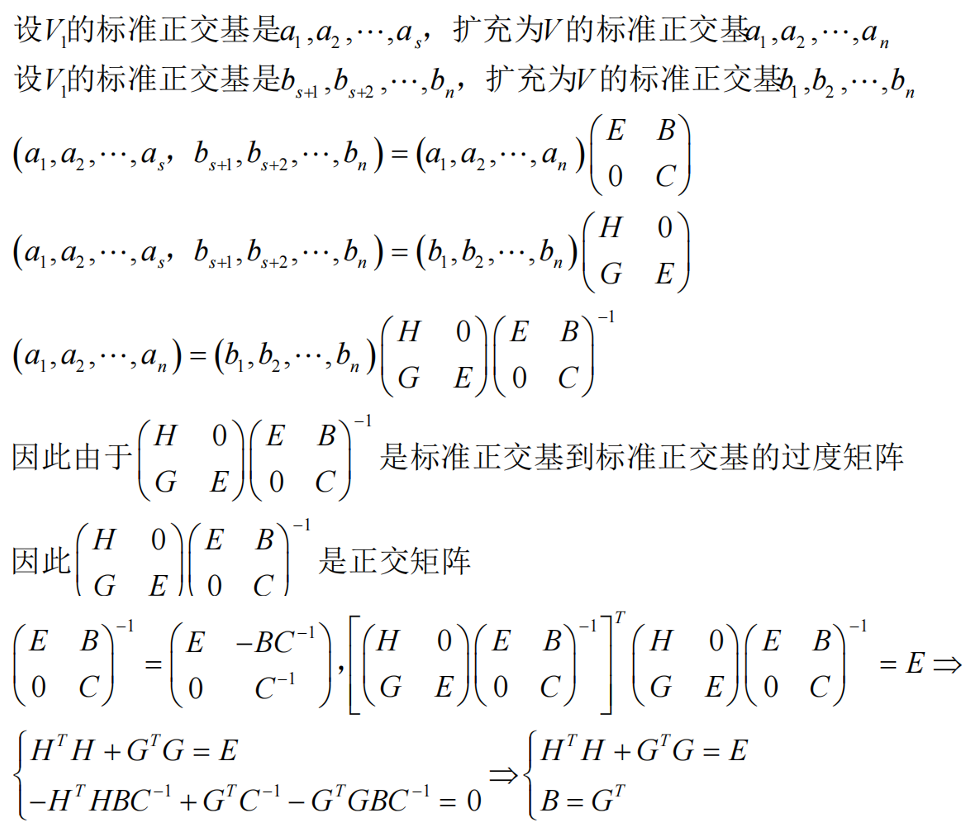
\includegraphics[scale=0.46]{3.png}
\end{figure}
\begin{figure}[htbp]
    \center
    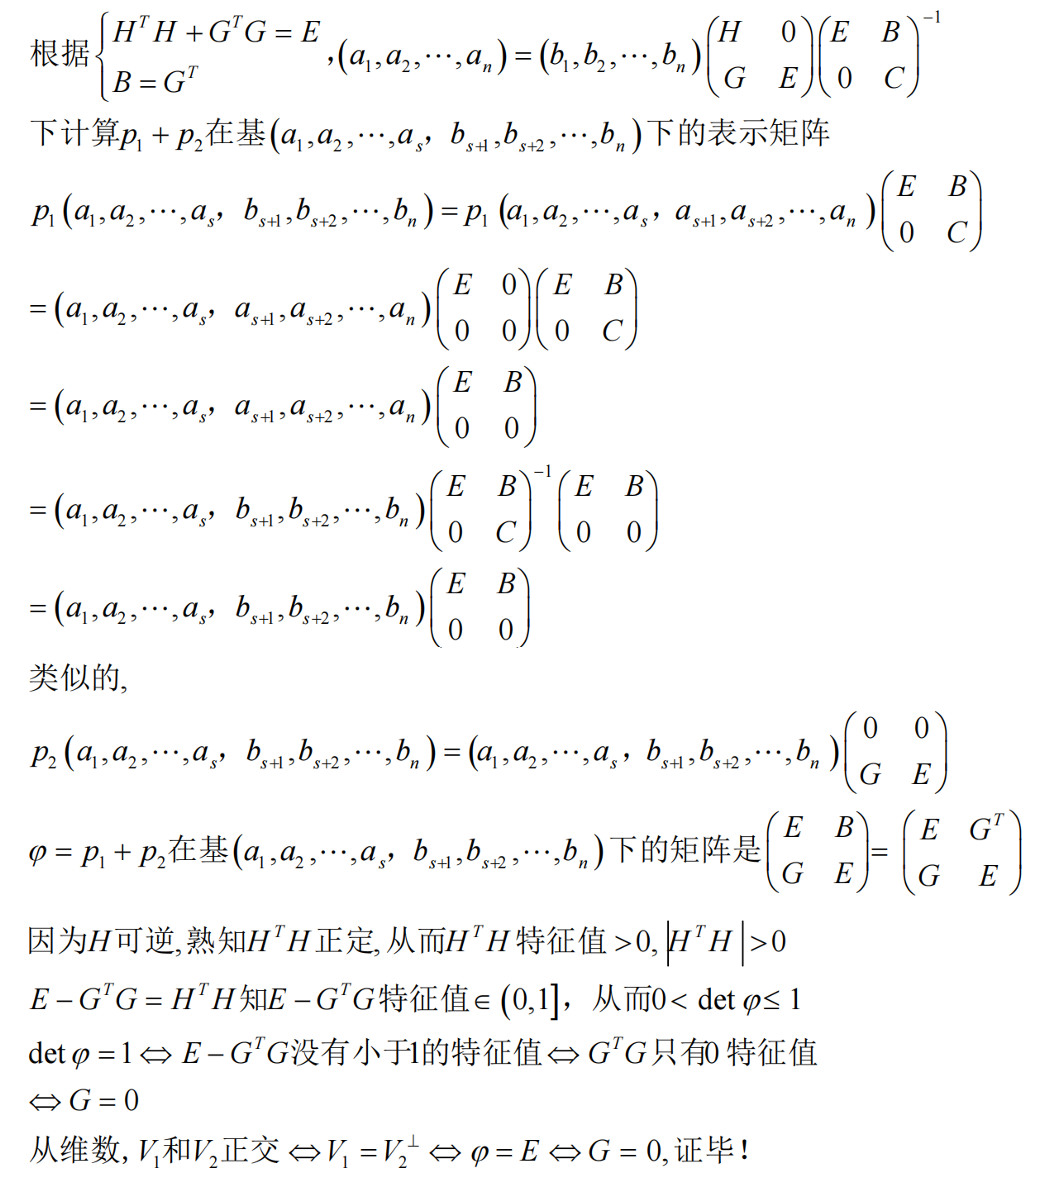
\includegraphics[scale=0.46]{4.png}
\end{figure}
\end{solution}
\end{document}